
\tikzset{every picture/.style={line width=0.75pt}} %set default line width to 0.75pt        

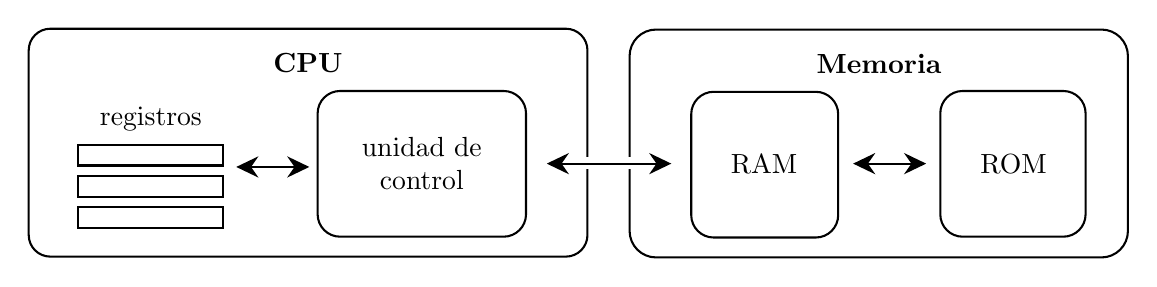
\begin{tikzpicture}[x=0.75pt,y=0.75pt,yscale=-1,xscale=1]
%uncomment if require: \path (0,300); %set diagram left start at 0, and has height of 300

%Rounded Rect [id:dp2413859954367672] 
\draw   (40.4,60.4) .. controls (40.4,54.66) and (45.06,50) .. (50.8,50) -- (299.2,50) .. controls (304.94,50) and (309.6,54.66) .. (309.6,60.4) -- (309.6,149.4) .. controls (309.6,155.14) and (304.94,159.8) .. (299.2,159.8) -- (50.8,159.8) .. controls (45.06,159.8) and (40.4,155.14) .. (40.4,149.4) -- cycle ;
%Shape: Rectangle [id:dp022760876802285557] 
\draw   (64.2,105.9) -- (134.2,105.9) -- (134.2,115.9) -- (64.2,115.9) -- cycle ;
%Shape: Rectangle [id:dp6765293736431461] 
\draw   (64.2,121.1) -- (134.2,121.1) -- (134.2,131.1) -- (64.2,131.1) -- cycle ;
%Shape: Rectangle [id:dp24942837973112963] 
\draw   (64.15,135.9) -- (134.15,135.9) -- (134.15,145.9) -- (64.15,145.9) -- cycle ;
%Rounded Rect [id:dp04827177357877366] 
\draw   (179.6,90.8) .. controls (179.6,84.84) and (184.44,80) .. (190.4,80) -- (269.2,80) .. controls (275.16,80) and (280,84.84) .. (280,90.8) -- (280,139.4) .. controls (280,145.36) and (275.16,150.2) .. (269.2,150.2) -- (190.4,150.2) .. controls (184.44,150.2) and (179.6,145.36) .. (179.6,139.4) -- cycle ;
%Rounded Rect [id:dp6285318603313554] 
\draw   (329.9,63.18) .. controls (329.9,56.12) and (335.62,50.4) .. (342.68,50.4) -- (557.22,50.4) .. controls (564.28,50.4) and (570,56.12) .. (570,63.18) -- (570,147.42) .. controls (570,154.48) and (564.28,160.2) .. (557.22,160.2) -- (342.68,160.2) .. controls (335.62,160.2) and (329.9,154.48) .. (329.9,147.42) -- cycle ;
%Rounded Rect [id:dp10015100458796722] 
\draw   (359.6,91.2) .. controls (359.6,85.24) and (364.44,80.4) .. (370.4,80.4) -- (419.6,80.4) .. controls (425.56,80.4) and (430.4,85.24) .. (430.4,91.2) -- (430.4,139.8) .. controls (430.4,145.76) and (425.56,150.6) .. (419.6,150.6) -- (370.4,150.6) .. controls (364.44,150.6) and (359.6,145.76) .. (359.6,139.8) -- cycle ;
%Rounded Rect [id:dp04449520492329406] 
\draw   (479.6,90.77) .. controls (479.6,84.82) and (484.42,80) .. (490.37,80) -- (538.83,80) .. controls (544.78,80) and (549.6,84.82) .. (549.6,90.77) -- (549.6,139.43) .. controls (549.6,145.38) and (544.78,150.2) .. (538.83,150.2) -- (490.37,150.2) .. controls (484.42,150.2) and (479.6,145.38) .. (479.6,139.43) -- cycle ;
%Straight Lines [id:da9625122316428356] 
\draw    (143.4,116.6) -- (172.6,116.6) ;
\draw [shift={(175.6,116.6)}, rotate = 180] [fill={rgb, 255:red, 0; green, 0; blue, 0 }  ][line width=0.08]  [draw opacity=0] (10.72,-5.15) -- (0,0) -- (10.72,5.15) -- (7.12,0) -- cycle    ;
\draw [shift={(140.4,116.6)}, rotate = 0] [fill={rgb, 255:red, 0; green, 0; blue, 0 }  ][line width=0.08]  [draw opacity=0] (10.72,-5.15) -- (0,0) -- (10.72,5.15) -- (7.12,0) -- cycle    ;
%Straight Lines [id:da12368584213082734] 
\draw    (440.6,115) -- (469.8,115) ;
\draw [shift={(472.8,115)}, rotate = 180] [fill={rgb, 255:red, 0; green, 0; blue, 0 }  ][line width=0.08]  [draw opacity=0] (10.72,-5.15) -- (0,0) -- (10.72,5.15) -- (7.12,0) -- cycle    ;
\draw [shift={(437.6,115)}, rotate = 0] [fill={rgb, 255:red, 0; green, 0; blue, 0 }  ][line width=0.08]  [draw opacity=0] (10.72,-5.15) -- (0,0) -- (10.72,5.15) -- (7.12,0) -- cycle    ;
%Shape: Rectangle [id:dp7915154307296417] 
\draw  [draw opacity=0][fill={rgb, 255:red, 255; green, 255; blue, 255 }  ,fill opacity=1 ] (303.4,111.8) -- (335.6,111.8) -- (335.6,117.8) -- (303.4,117.8) -- cycle ;
%Straight Lines [id:da2756585120657784] 
\draw    (293,115) -- (347,115) ;
\draw [shift={(350,115)}, rotate = 180] [fill={rgb, 255:red, 0; green, 0; blue, 0 }  ][line width=0.08]  [draw opacity=0] (10.72,-5.15) -- (0,0) -- (10.72,5.15) -- (7.12,0) -- cycle    ;
\draw [shift={(290,115)}, rotate = 0] [fill={rgb, 255:red, 0; green, 0; blue, 0 }  ][line width=0.08]  [draw opacity=0] (10.72,-5.15) -- (0,0) -- (10.72,5.15) -- (7.12,0) -- cycle    ;

% Text Node
\draw (175,66.35) node   [align=left] {\begin{minipage}[lt]{170.54pt}\setlength\topsep{0pt}
\begin{center}
\textbf{CPU}
\end{center}

\end{minipage}};
% Text Node
\draw (99.28,93.65) node   [align=left] {\begin{minipage}[lt]{47.77pt}\setlength\topsep{0pt}
\begin{center}
registros
\end{center}

\end{minipage}};
% Text Node
\draw (229.8,114.7) node   [align=left] {\begin{minipage}[lt]{68.44pt}\setlength\topsep{0pt}
\begin{center}
unidad de control
\end{center}

\end{minipage}};
% Text Node
\draw (450.08,67.15) node   [align=left] {\begin{minipage}[lt]{163.1pt}\setlength\topsep{0pt}
\begin{center}
\textbf{Memoria}
\end{center}

\end{minipage}};
% Text Node
\draw (394.69,115.1) node   [align=left] {\begin{minipage}[lt]{48.14pt}\setlength\topsep{0pt}
\begin{center}
RAM
\end{center}

\end{minipage}};
% Text Node
\draw (514.91,115.1) node   [align=left] {\begin{minipage}[lt]{47.6pt}\setlength\topsep{0pt}
\begin{center}
ROM
\end{center}

\end{minipage}};


\end{tikzpicture}
